\subsubsection{GRU Results}

\begin{table}[H]
\centering
\caption{Classification Report for GRU model using CLS token embeddings}
\label{tab:gru_classification_report}
\begin{tabular}{lcccc}
\toprule
Class        & Precision & Recall & F1-score & Support \\
\midrule
0            & 0.87      & 0.93   & 0.90     & 4953    \\
1            & 0.92      & 0.87   & 0.89     & 5084    \\
\midrule
Accuracy     &           &        & 0.90     & 10037   \\
Macro Avg    & 0.90      & 0.90   & 0.90     & 10037   \\
Weighted Avg & 0.90      & 0.90   & 0.90     & 10037   \\
\bottomrule
\end{tabular}
\end{table}

\begin{figure}[H]
    \centering
    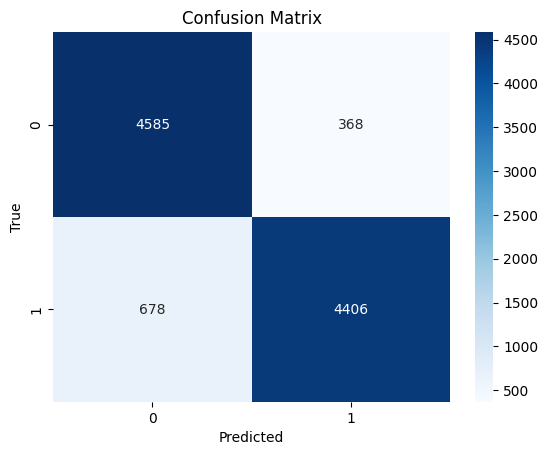
\includegraphics[width=0.45\textwidth]{images/confusion_matrix_gru.png}
    \caption{Confusion matrix for GRU model using CLS embeddings}
    \label{fig:confusion_gru}
\end{figure}

\begin{figure}[H]
    \centering
    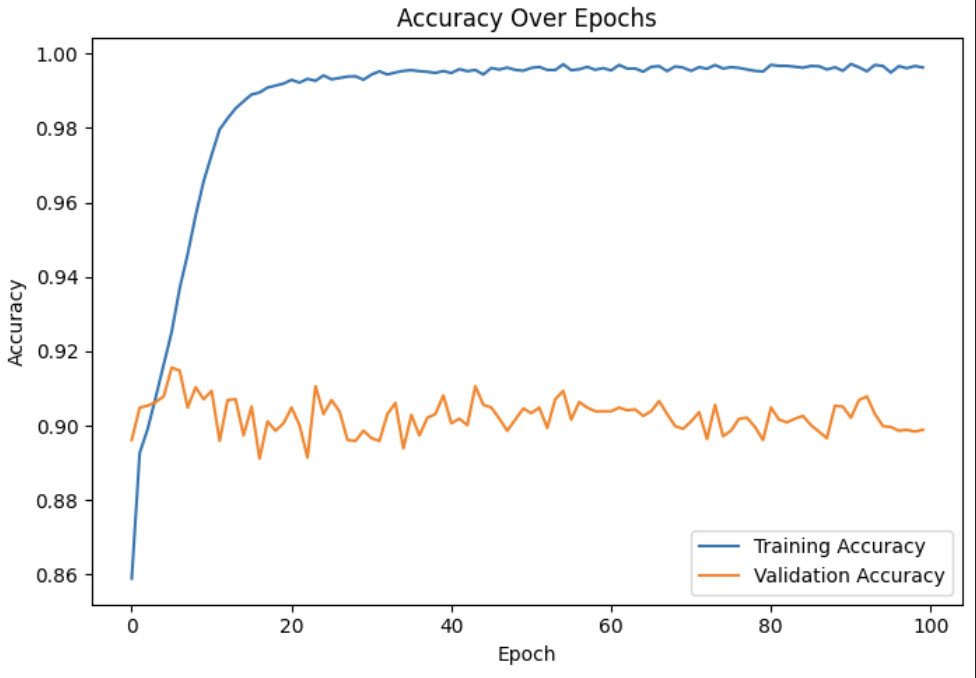
\includegraphics[width=0.45\textwidth]{images/accuracy_over_epoch_gru.png}
    \caption{Accuracy over epochs for the GRU model.}
    \label{fig:accuracy_gru}
\end{figure}

\begin{figure}[H]
    \centering
    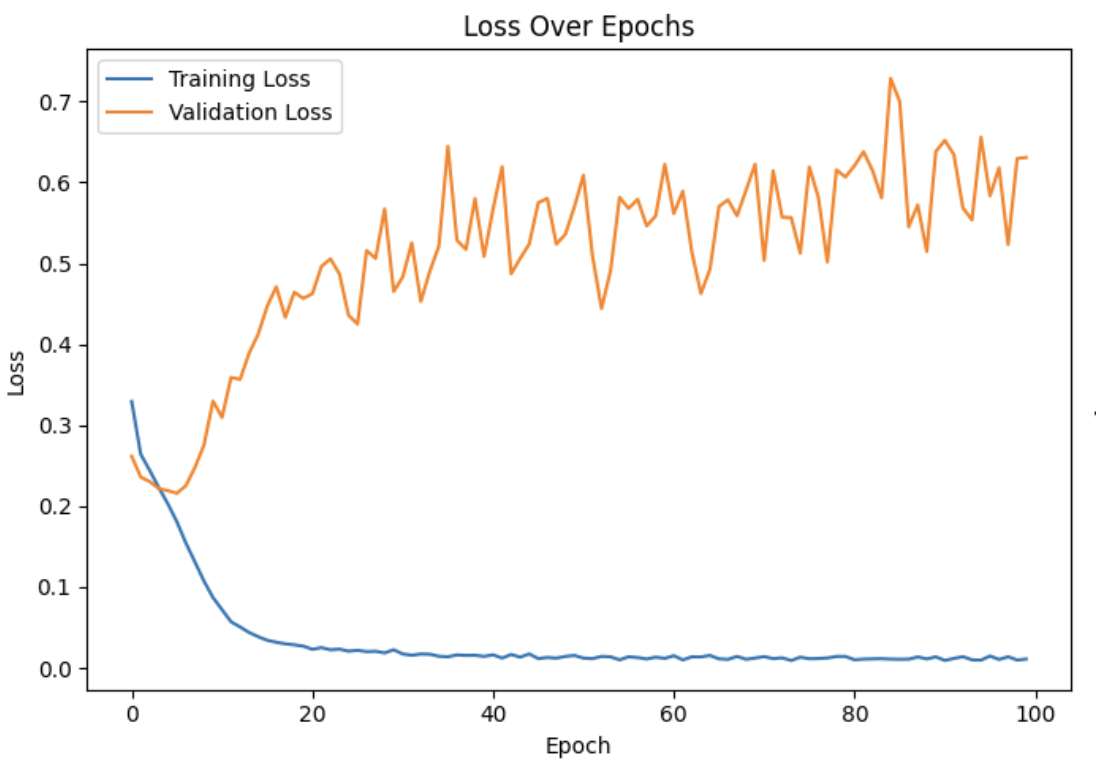
\includegraphics[width=0.45\textwidth]{images/lossOverEpochGRU.png}
    \caption{Loss over epochs for the GRU model.}
    \label{fig:loss_gru}
\end{figure}


\begin{figure}[H]
    \centering
    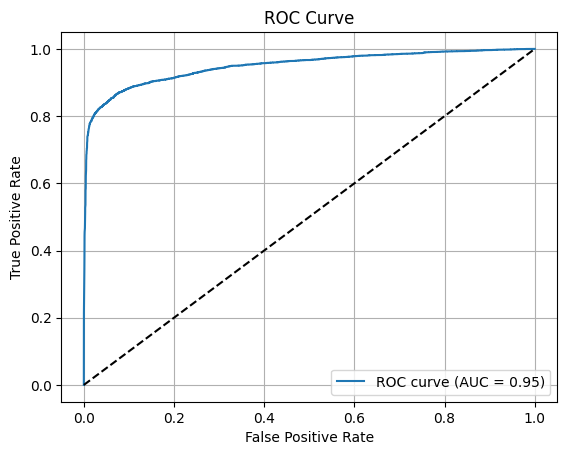
\includegraphics[width=0.45\textwidth]{images/roc_curve_gru.png}
    \caption{ROC curve for GRU model}
    \label{fig:roc_gru}
\end{figure}

\begin{figure}[H]
    \centering
    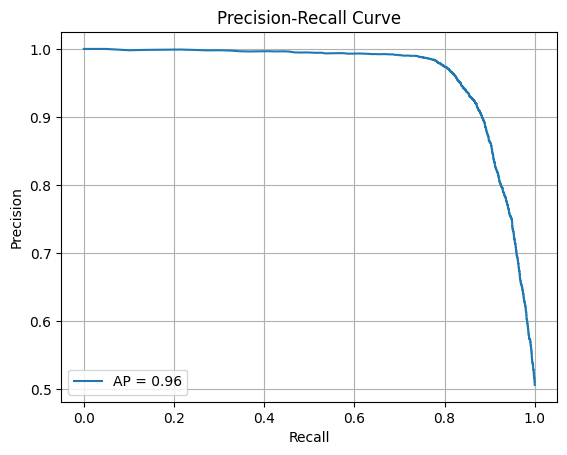
\includegraphics[width=0.45\textwidth]{images/precision_recall_gru.png}
    \caption{Precision-Recall curve for GRU model with AP = 0.96}
    \label{fig:pr_gru}
\end{figure}

The GRU model trained on CLS token embeddings demonstrated strong classification performance, achieving an overall accuracy of 90\% and an F1-score of 0.89 for the hate speech class (Table~\ref{tab:gru_classification_report}). The model showed balanced performance across both classes, with precision and recall values above 0.87. The confusion matrix in Figure~\ref{fig:confusion_gru} illustrates this balance, with 4585 true negatives and 4406 true positives, though 678 hate examples were misclassified as non-hate.

Despite the strong predictive performance, the training curves in Figure~\ref{fig:accuracy_gru} and Figure~\ref{fig:loss_gru} indicate potential overfitting. The training loss decreases consistently, but the validation loss remains high and fluctuates significantly across epochs. Similarly, the training accuracy approaches 99\% while validation accuracy stabilizes near 90\%, suggesting that the model has learned the training data very well but may not generalize perfectly to unseen data.

Nevertheless, the ROC curve in Figure~\ref{fig:roc_gru} shows excellent separability between classes, with an AUC close to 0.93. The Precision-Recall curve in Figure~\ref{fig:pr_gru} further supports this, with an average precision (AP) of 0.96, indicating that the model maintains high precision across a wide range of recall thresholds. These metrics confirm that the GRU model is effective at ranking and identifying hate speech with high confidence, even under class imbalance conditions.